\chapter{指令}
\section{引言}
\paragraph{指令集}~{一个给定的计算机体系结构所包含的指令集合} 
\paragraph{汇编语言和机器语言}~{前者是编程的书写形式, 后者是计算机所能识别的形式} 
\paragraph{存储程序}~{多种类型的指令和数据均以数字形式存储在存储器(内存)中}
\paragraph{MIPS}~{是一种汇编语言, 属于精简指令集}
\section{硬件操作}
\subsection{MIPS汇编指令}
\begin{itemize}
\item 每条MIPS算数运算指令只执行一个操作
\item 一行写一条命令
\item \#后是注释
\end{itemize}
\subsection{高级语言与编译语言之间的关系}
高级语言经过编译器编译, 形成汇编语言.
\section{MIPS寄存器及常用指令}
高级语言的变量数量不受限制, 而汇编语言逻辑运算指令的变量对应寄存器, 而寄存器数量有限, 故变量数量受限.
\subsection{寄存器}
\begin{itemize}
\item 共有\verb|32|个寄存器, 编号为\verb|0-31|
\item \verb|32bit|数据称为一个``字'', \verb|32|位为字长, 每个字\verb|4|字节
\item 按字节编址
\item 寄存器分类型:
\begin{itemize}
\item \verb|$ZERO|: 恒为\verb|0|
\item \verb|$v0-$v1|: 返回值
\item \verb|$a0-$a3|: 参数
\item \verb|$t0-$t9|: 临时变量, 其中\verb|$t0-$t7|对应编号\verb|8-15|, \verb|$t8-$t9|对应编号\verb|24-25|, 无需压栈
\item \verb|$s0-$s7|: 保留变量, 对应编号\verb|16-23|, 必须压栈
\item \verb|$gp|: 静态数据的全局指针
\item \verb|$sp|: 栈指针
\item \verb|$fp|: 帧指针
\item \verb|$ra|: 返回地址
\end{itemize}
\end{itemize}
\subsection{常见指令}
复杂的数据结构(数组等)存储于存储器中, 需要用数据传输指令交换数据:
\begin{itemize}
\item \verb|lw rt, shamt(rs)|: 取数
\item \verb|sw rs, shamt(rt)|: 存数
\end{itemize}\par
数据被存储到寄存器后, 可以进行相加减:
\begin{itemize}
\item \verb|add rd, rs, rt|: 加法
\item \verb|sub rd, rs, rt|: 减法
\end{itemize}\par
我们经常要在加减运算的时候用到常数, 这样就会导致计算机会去内存中取出这个常数存储到寄存器这一多余的步骤, 可以通过立即数以除去这一过程:
\begin{itemize}
\item \verb|addi rt, rs, constant|: 加立即数
\item \verb|-addi rt, rs, constant|: 没有减立即数, 用这个替代
\end{itemize}\par 
特殊的, 如果我们要进行寄存器间的赋值, 可以通过\verb|add|或者\verb|addi|实现:
\begin{itemize}
\item \verb|add rd, rs, $ZERO|: 将\verb|rs|赋值给\verb|rd|
\item \verb|addi rt, rs, 0|: 将\verb|rs|赋值给\verb|rt|
\end{itemize}
\section{MIPS指令格式}
指令包含操作码和地址码.
\subsection{R型指令}
\begin{table}[H]
\centering
\begin{tabularx}{\textwidth}{|Z|Z|Z|Z|Z|Z|}
\hline
op & rs & rt & rd & shamt & funct  \\
\hline
\end{tabularx}
\end{table} \par 
他们的作用:
\begin{itemize}
\item \verb|op|: 操作码
\item \verb|rs|: 第一个源寄存器号
\item \verb|rt|: 第二个源寄存器号
\item \verb|rd|: 目标寄存器号
\item \verb|shamt|: 位移量
\item \verb|funct|: 功能码(与\verb|op|一起起作用)
\end{itemize} \par 
他们的位数:
\begin{itemize}
\item \verb|op|: \verb|6|位, 因为有\verb|64|种指令
\item \verb|rs,rt,rd|: \verb|5|位, 因为有\verb|32|个寄存器
\item \verb|shamt|: \verb|5|位, 因为MIPS是\verb|32|位指令
\item \verb|funct|: \verb|6|位, 因为\verb|32-6-5-5-5-5=6|
\end{itemize}\par
上述操作码可以查询表格, 寄存器号需要记忆, 下面也一样.
\subsection{I型指令}
\begin{table}[H]
\centering
\begin{tabularx}{\textwidth}{|Z|Z|Z|p{15em}<{\centering}|}
\hline
op & rs & rt & constant or address \\
\hline
\end{tabularx}
\end{table}\par
他们的作用:
\begin{itemize}
\item \verb|op|: 操作码
\item \verb|rs|: 源寄存器号
\item \verb|rt|: 目标寄存器号
\item \verb|constant or address|: 偏移量
\end{itemize}\par
他们的位数:
\begin{itemize}
\item \verb|op|: \verb|6|位, 因为有\verb|64|种指令
\item \verb|rs,rt|: \verb|5|位, 因为有\verb|32|个寄存器
\item \verb|constant or address|: \verb|16|位, 因为\verb|32-6-5-5=16|
\end{itemize}
\subsection{J型指令}
\begin{table}[H]
\centering
\begin{tabularx}{\textwidth}{|Z|Z|}
\hline
op & address \\
\hline
\end{tabularx}
\end{table}\par
他们的作用:
\begin{itemize}
\item \verb|op|: 操作码
\item \verb|address|: 地址
\end{itemize}\par
他们的位数:
\begin{itemize}
\item \verb|op|: \verb|6|位, 因为有\verb|64|种指令
\item \verb|address|: \verb|26|位, 因为\verb|32-6=26|
\end{itemize}
\section{MIPS逻辑操作}
\subsection{指令}
逻辑移动指令:
\begin{itemize}
\item \verb|sll rd, rt, shamt|: 逻辑左移指令, \verb|rt|中的数左移\verb|shamt|位, 空出的位补\verb|0|, 结果存\verb|rd|
\item \verb|srl rd, rt, shamt|: 逻辑右移指令, \verb|rt|中的数右移\verb|shamt|位, 空出的位补\verb|0|, 结果存\verb|rd|
\end{itemize}\par
上述指令为R型指令, 其中\verb|op|都为\verb|0|, \verb|func|分别为\verb|0|和\verb|6|, \verb|shamt|为位移量, \verb|rs|不使用为0. \par
逻辑运算指令:
\begin{itemize}
\item \verb|add rd, rs, rt|: 逻辑与指令, \verb|rs|和\verb|rt|按位与, 结果存\verb|rd|
\item \verb|or rd, rs, rt|: 逻辑或指令, \verb|rs|和\verb|rt|按位或, 结果存\verb|rd|
\item \verb|nor rd, rs, rt|: 逻辑或非指令, \verb|rs|和\verb|rt|按位或非, 结果存\verb|rd|
\end{itemize}\par
上述指令为R型指令, \verb|op|都为\verb|0|, \verb|func|分别为\verb|20|,\verb|25|,\verb|27|, \verb|shamt|全为\verb|0|.
\section{MIPS决策指令}
\subsection{指令}
\verb|bne|和\verb|beq|指令:
\begin{itemize}
\item \verb|beq rs, rt, L1|: 如果\verb|rs=rt|跳转到标签为\verb|L1|的指令
\item \verb|bne rs, rt, L1|: 如果\verb|rs!=rt|跳转到标签为\verb|L1|的指令
\item \verb|j L1|: 无条件转移到标签为\verb|L1|的指令
\end{itemize}\par
前两条为I型指令, \verb|op|分别为\verb|4|,\verb|5|,\verb|2|. 最后一条指令为J型指令.\par
\verb|slt|和\verb|slti|指令:
\begin{itemize}
\item \verb|slt $rd, $rs, $rt|: 若\verb|rs<rt|, 则\verb|rd=1|, 否则\verb|rd=0|
\item \verb|slti $rt, $rs, constant|: 若\verb|rs<constant|, 则\verb|rd=1|, 否则\verb|rd=0|
\end{itemize}
\subsection{条件分支代码转MIPS}
将以下代码:
\begin{lstlisting}
# f,g,h,i,j存储于$s0,$s1,$s2,$s3,$s4
if (i == j) f = g + h;
else f = g - h;
\end{lstlisting}\par
转换为MIPS:
\begin{lstlisting}
       bne $s3, $s4 ELSE
       add $s0, $s1, $s2
       j EXIT
ELSE: $s0, $s1, $s2
EXIT: ...
\end{lstlisting}
\subsection{循环代码转MIPS}
将以下代码:
\begin{lstlisting}
while (save[i] == k) i += 1; # i存于$s3, k存于$s5, save的基址存于$s6
\end{lstlisting}\par
转为MIPS:
\begin{lstlisting}
LOOP: sll $t0, $s3, 2 # $t0 = i * 4, 找到地址
       add $t0, $s6, $t0 # $t0 = 基址 + 偏移量
       lw $t1, 0($t0) # 从内存中取出数存到$t1
       bne $t1, $s5, EXIT # 若和k不相等退出
       addi $s3, $s3, 1 # 循环体
       j LOOP # 实现循环
EXIT: ...
\end{lstlisting}
\section{MIPS函数}
\subsection{指令}
\begin{itemize}
\item \verb|jal Address|: 跳转到函数地址, 并将\verb|PC+4|存储于\verb|$ra|以便返回断点处
\item \verb|jr $ra|: 返回断点处
\end{itemize}
\subsection{栈}
我们使用任何寄存器需要保存它原来的值(类似于中断保存现场), 用完了再把原来的值放回去, 因为寄存器的数量是有限的. \par 
一般来说, \verb|$s|开头的寄存器必须压栈, \verb|$t|/\verb|$a|开头的寄存器不必压栈.
\subsubsection{压栈和出栈}
由于栈的增长是按地址从高到低的顺序进行的, 所以出栈和入栈的操作分别为:
\begin{enumerate}
\item 入栈(\verb|push|): \verb|$sp=$sp-4|
\item 出栈(\verb|pop|): \verb|$sp=$sp+4|
\end{enumerate}
\subsection{函数代码转MIPS}
将以下代码:
\begin{lstlisting}
int leaf_example (int g, h, i, j)
{
    int f;
    f = (g + h) - (i + j);
    return f;
}
\end{lstlisting}\par
转换为MIPS:
\begin{lstlisting}
# 入栈
addi $sp, $sp, -12
sw $t1, 8($sp)
sw $t0, 4($sp)
sw $s0, 0($sp)
# 运算
add $t0, $a0, $a1
add $t1, $a2, $a3
add $s0, $t0, $t1
addi $v0, $s0, $ZERO # 将结果$s0放到函数返回值寄存器$v0
# 出栈
lw $s0, 0($sp)
lw $t0, 4($sp)
lw $t1, 8($sp)
addi $sp, $sp, 12
# 返回
jr $ra
\end{lstlisting}
\section{MIPS嵌套}
不调用其他过程的过程称为\textbf{叶过程}, 嵌套调用就是过程体中调用其他的过程(甚至包括自己) \par
首先要知道, 递归分为两个阶段: 递归阶段和返回阶段. \par
假设主程序将参数\verb|3|传入寄存器\verb|$a0|, 然后使用\verb|jal A|调用过程\verb|A|. 再假设过程\verb|A|通过\verb|jal B|调用过程\verb|B|, 参数为\verb|7|, 同样存入\verb|$a0|. 由于\verb|A|尚未完成任务, 所以寄存器\verb|$a0|的使用上存在冲突. 同样, 在寄存器\verb|$ra|保存的返回地址上也存在冲突, 因为它现在保存的是\verb|B|的返回地址. 所以我们必须采用压栈的方式对数据进行保存: \par
Caller把所有在返回阶段需要用到的参数寄存器(\verb|$a0-$a3|)或临时寄存器\verb|$t0-$t9|压栈. Callee把将所有在返回阶段要用到的返回地址寄存器\verb|$ra|和保存寄存器\verb|$s0-$s7|都压栈. 栈指针\verb|$sp|会随诊栈中寄存器的个数调整. 到返回的时候, 寄存器就会从存储器中恢复, 栈指针也会重新调整.
\subsection{递归代码转MIPS}
将以下代码:
\begin{lstlisting}
int fact(int n)
{
    if (n < 1) return (1);
        else return (n * fact(n - 1));
}
\end{lstlisting}\par
转换为MIPS:
\begin{lstlisting}
fact:
      addi $sp, $sp, -8
      sw $ra, 4($sp)
      sw $a0, 0($sp)
      slti $t0, $a0, 1
      beq $t0, $ZERO, L1
      addi $v0, $ZERO, 1
      addi $sp, $sp, 8
      jr $ra
      # 申请一块大小为8的空间
      # 将返回阶段要用到的Caller的返回地址存储到栈
      # 将返回阶段要用到的Callee的参数存储到栈
      # 如果$a0也就是n大于等于1, 则跳到L1
      # 如果$a0也就是n小于1, 则递归阶段到达最底层, 计算0!=1并保存结果
      # 由于是最底层函数, 其$ra和$a0不会被下一层调用, 所以可以直接释放栈
      # 最底层函数返回
L1:
      addi $a0, $a0, -1
      jal fact
      lw $a0, 0($sp)
      lw $ra, 4($sp)
      addi $sp, $sp, 8
      mul $v0, $a0, $v0
      jr $ra
      # 设置下一层调用函数的参数为n-1
      # 返回fact, 执行fact(n-1)
      # 开始返回阶段, 将递归阶段存储的$a0取出
      # 开始返回阶段, 将递归阶段存储的$ra取出
      # 释放栈
      # 根据刚取出的$a0和$v0相乘
      # 函数返回
\end{lstlisting}\par 
过程示意图:
\begin{figure}[H]
\centering
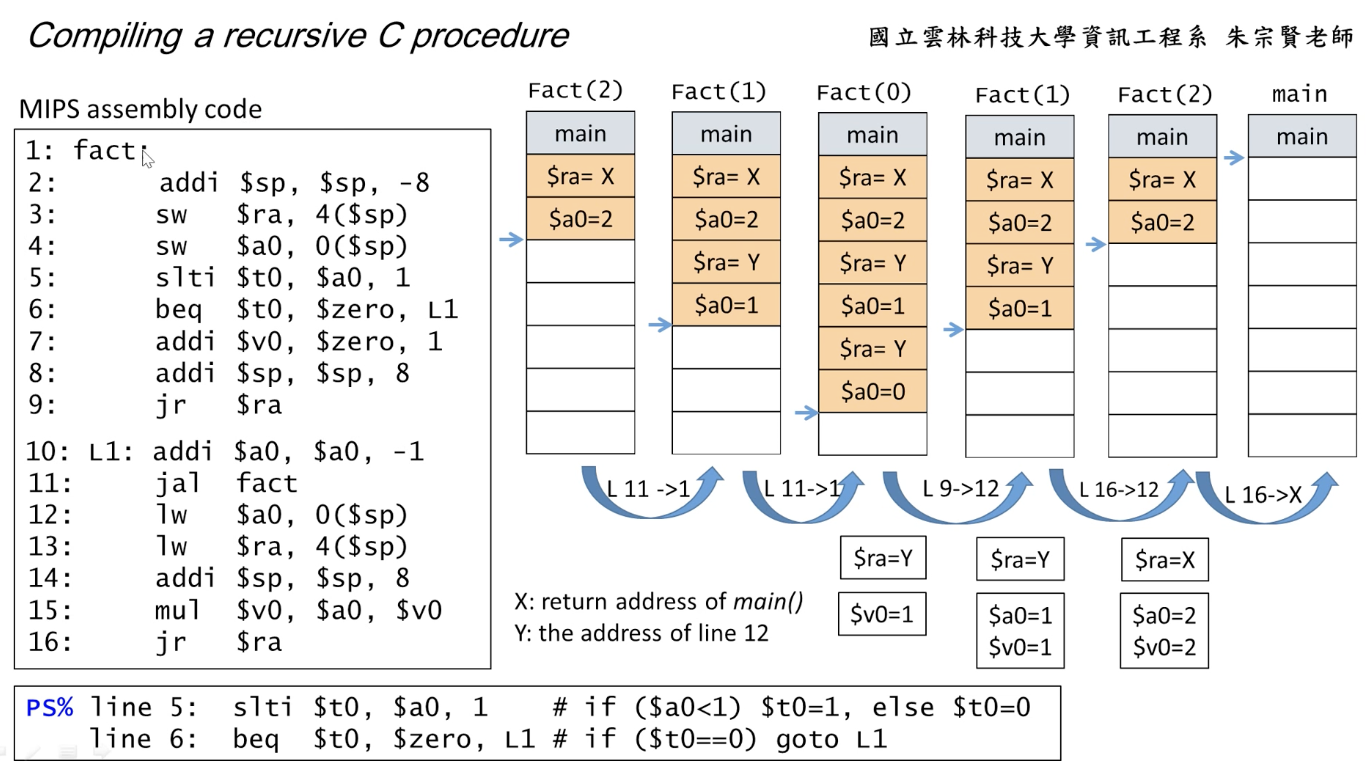
\includegraphics[scale=.5]{img/figure2.png}
\end{figure}
\section{寻址方式}
寻址方式就是根据地址找到指令或者操作数的方法. \par 假设有数据存储在地址为\verb|EA|的内存中, 用\verb|()|表示内存的内容:
\begin{enumerate}
\item 直接寻址: 指令中的形式地址\verb|A|就是真实地址\verb|EA|, 即\verb|A|=\verb|EA|
\begin{figure}[H]
\centering
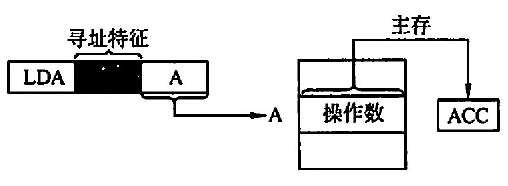
\includegraphics[scale=.9]{img/figure3.png}
\end{figure}
\item 间接寻址: 指令中的形式地址\verb|A|是真实地址的地址, 即\verb|(A)=EA|
\begin{figure}[H]
\centering
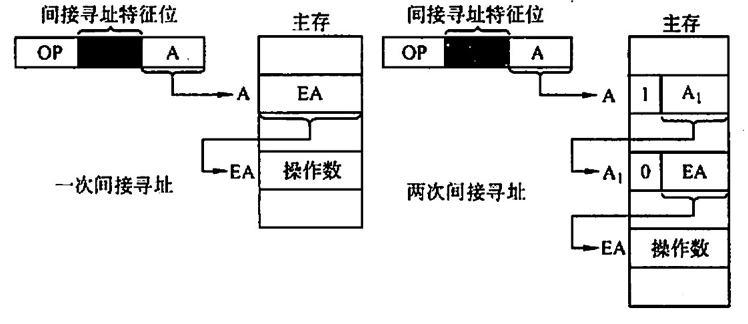
\includegraphics[scale=.9]{img/figure4.png}
\end{figure}
\item 寄存器寻址: 指令中的地址是寄存器号\verb|Ri|, 寄存器中存储了操作数, 即\verb|Ri=EA|
\begin{figure}[H]
\centering
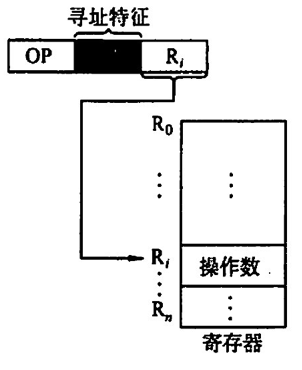
\includegraphics[scale=.9]{img/figure5.png}
\end{figure}
\item 寄存器间接寻址: 指令中的地址是寄存器号\verb|Ri|, 寄存器中存储了真实地址\verb|EA|, 即\verb|(Ri)=EA|
\begin{figure}[H]
\centering
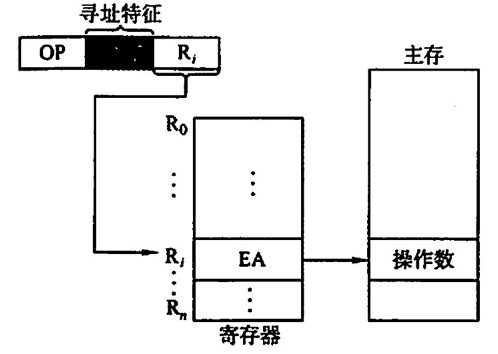
\includegraphics[scale=.9]{img/figure6.png}
\end{figure}
\item 相对寻址: 将程序计数器\verb|PC|的内容和指令中的形式地址\verb|A|相加得到真实地址\verb|EA|, 即\verb|(PC)+A=EA|
\begin{figure}[H]
\centering
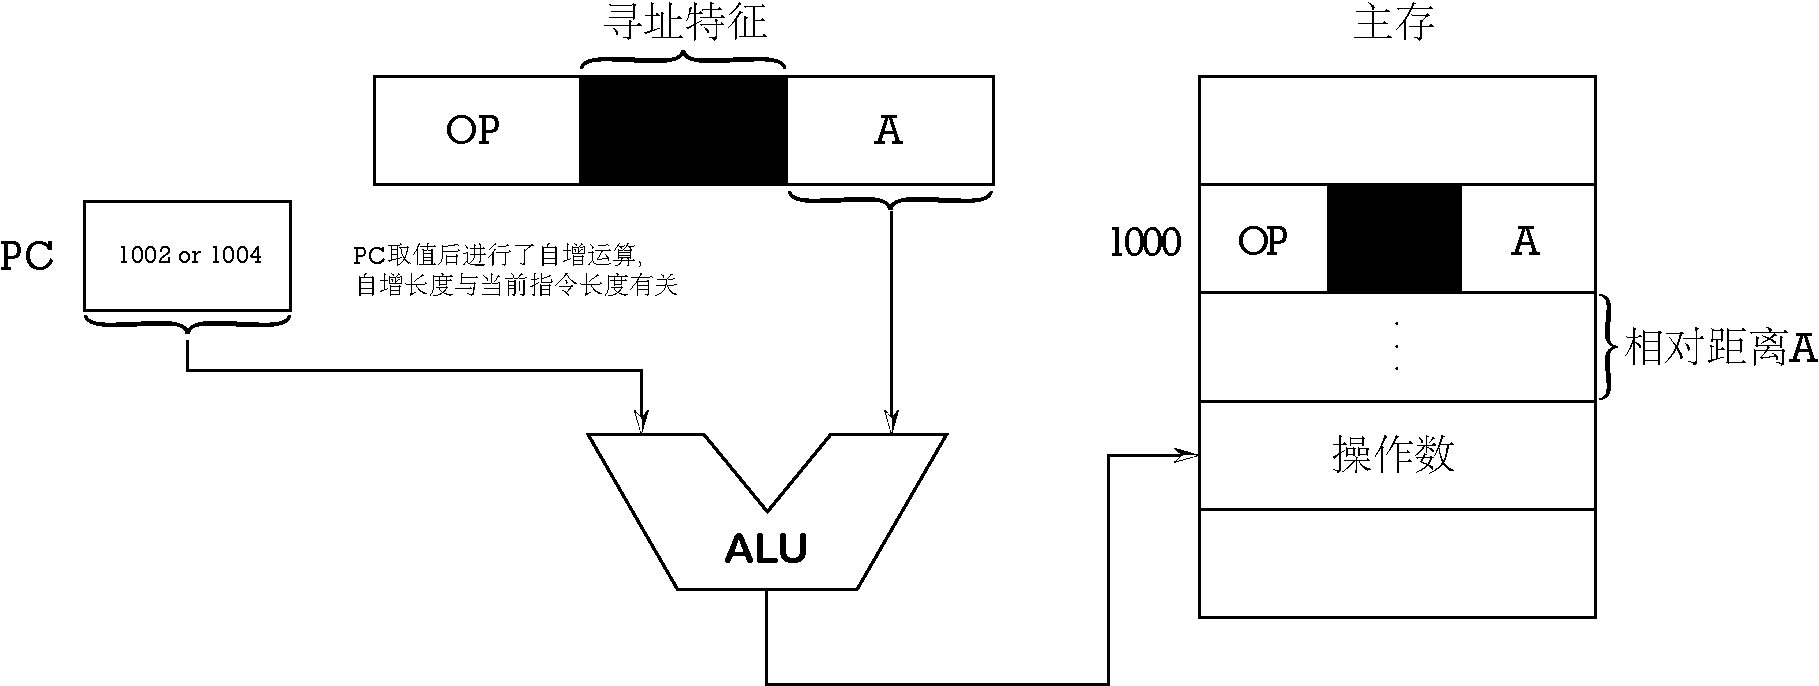
\includegraphics[scale=.9]{img/figure7}
\end{figure}
\item 基址寻址: 将基址寄存器\verb|BR|的内容和指令中的形式地址\verb|A|相加得到真实地址\verb|EA|, 即\verb|(BR)+A=EA|
\begin{figure}[H]
\centering
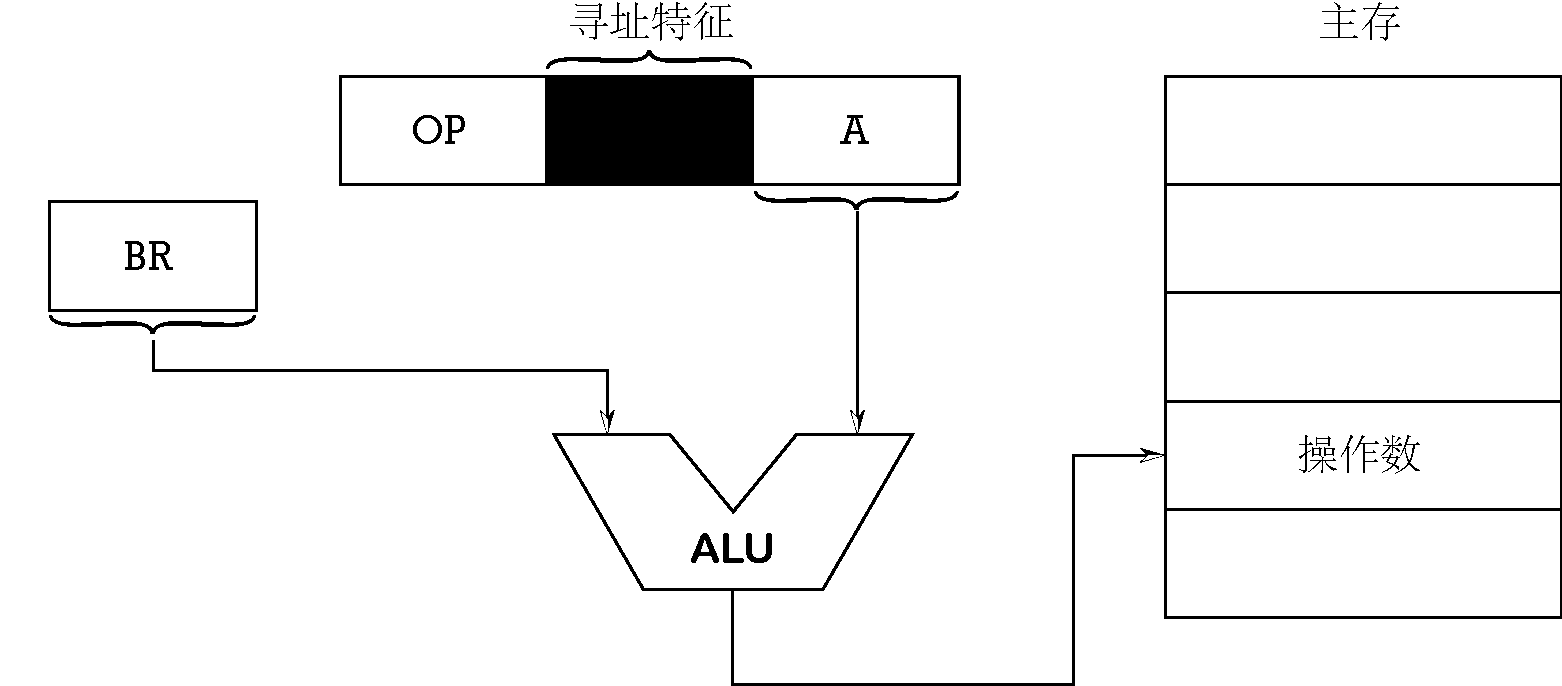
\includegraphics[scale=.9]{img/figure8}
\end{figure}
\end{enumerate}
\chapter{运算}
\section{进位计数制}
\subsection{进位计数法}
\verb|r|进制数, 每个数码位可能出现\verb|r|种字符, 逢\verb|r|进\verb|1|.
\subsection{不同进制数之间的转换}
\subsubsection{\texttt{r}进制数$ \rightarrow $十进制}
各数码位与位权的乘积之和, 全为\verb|1|的二进制转十进制: \verb|2^n-1|
\subsubsection{十进制$ \rightarrow $ \texttt{r}进制}
\begin{itemize}
\item 整数部分: 除基取余法, 先取得的``余''是整数的低位(除\verb|r|)
\item 小数部分: 乘基取整法, 先取得的``整''是消暑的高位(乘\verb|r|)
\end{itemize}
\subsubsection{二进制$ \leftrightarrow $八进制}
每三个二进制位对应一个八进制位
\subsubsection{二进制$ \leftrightarrow $十六进制}
每四个二进制位对应一个十六进制位
\section{定点数的表示}
\subsection{数的分类}
\begin{itemize}
\item 有符号数
\begin{itemize}
\item 定点数: 小数点位置固定的数
\begin{itemize}
\item 定点整数: 纯整数
\item 定点小数: 纯小数
\end{itemize}
\item 浮点数: 小数点位置不定的数(既有整数又有小数)
\end{itemize}
\item 无符号数(如地址)
\end{itemize}
\subsection{真值和机器数}
\begin{itemize}
\item 真值: 实际带正负号的数值(人类习惯的样子)
\item 机器数: 把正负号数字化的数(存到机器里的样子), 包括原码, 反码, 补码, 移码, 他们都是有符号数
\end{itemize}
\subsection{原码}
\begin{enumerate}
\item 含义 \par
用尾数表示真值的绝对值, 符号位``0/1''对应``正/负''. 若机器字长为\verb|n+1|位, 则尾数就占\verb|n|位.
\item 范围 \par
\verb|0|表示不唯一, (\verb|[+0]原=0,0000000,[-0]原=1,000000|), 范围为\verb|-2^n-1~2^n-1|, \verb|n|为尾数长度
\item 示例 \par
机器字长为\verb|8|位, 将真值\verb|x=-14|转换为原码: \verb|[x]原=1,0001110|(注意: 不足的机器字长要补\verb|0|)
\end{enumerate}
\subsection{反码}
\begin{enumerate}
\item 含义 \par
\begin{itemize}
\item 正数: 与原码相同
\item 负数: 符号位不变, 数值位取反
\end{itemize}
\item 范围 \par
\verb|0|表示方法不唯一, (\verb|[+0]反=0,0000000, [-0]反=1,1111111|), 范围为\verb|-2^n-1~2^n-1|, \verb|n|为尾数长度
\item 示例 \par
机器字长为\verb|8|位, 将真值\verb|x=-14|转换为反码: \verb|[x]反=1,1110001|
\end{enumerate}
\subsection{补码}
\begin{enumerate}
\item 含义 \par
先将原码转化为反码, 再将数值位\verb|+1|. \par 或者, 将原码直接转为补码: 从后往前, 遇到的第一个\verb|1|之前不变, 后面取反(符号位不变), 反过来补码转原码也是如此.
\item 范围 \par
\verb|0|的表示方法唯一, (\verb|[0]=0,0000000, 1,0000000用于表示-128|), 范围为\verb|-2^n~2^n-1|, \verb|n|为尾数长度
\item 示例 \par
机器字长为\verb|8|位, 将真值\verb|x=-14|转换为补码: 原码为\verb|[x]原=1,0001110|, 从右往左第一个\verb|1|不变, 左边取反, 得到补码\verb|[x]补=1,1110010|
\end{enumerate} \par 比较这两个数字的大小: \verb|1,1111111|和\verb|1,0000000|, 前者大, 因为前者转换为真值是\verb|1|, 而后者转化为真值为\verb|-128|
\subsection{移码}\label{移码}
移码与原码, 反码, 补码不同, 他是一种无符号数. \par 移码=真值+偏置值, 若机器字长为\verb|n+1|位, 则偏置值为\verb|+2^n|, 当偏置值为\verb|+128|的时候: 补码=补码的符号位取反. \par
偏置值可以取其他值, 如在\hyperref[IEEE 754]{\texttt{IEEE 754}}中, 单精度浮点数的偏移量为\verb|+127|, 即\verb|+01111111|.
\section{定点数的运算}
\subsection{移位运算} % TODO 移位运算的溢出问题
左移相当于\verb|*2|, 右移相当于\verb|/2|
\begin{itemize}
\item 逻辑移位: 无符号数, 当成正数, 补\verb|0|
\item 算术移位: 有符号数, 有正有负
\begin{itemize}
\item 正数: 符号位不参与移位, 原码, 反码, 补码数值位均补\verb|0|
\item 负数: 符号位不参与移位, 原码补\verb|0|, 反码补\verb|1|, 补码如果是左移, 补\verb|0|; 如果是右移, 补\verb|1|
\end{itemize}
\end{itemize} \par
左移: 若舍弃的位为\verb|1|, 将产生严重误差; \par 右移: 若舍弃的位为\verb|1|, 将丢失精度.
\subsection{加减运算}
\begin{itemize}
\item 原码的加减运算
\begin{itemize}
\item 加法运算
\begin{itemize}
\item 正+正: 绝对值做加法, 符号位为\verb|0|
\item 负+负: 绝对值做加法, 符号位为\verb|1|
\item 正+负: 绝对值大的减绝对值小的, 符号位同绝对值大的数
\item 负+正: 绝对值大的减绝对值小的, 符号位同绝对值大的数
\end{itemize}
\item 减法运算: 减数的符号位取反, 转变为加法
\end{itemize}
\item 补码的加减运算
\begin{itemize}
\item 加法运算: \verb|[A+B]补=[A]补+[B]补|
\item 减法运算: \verb|[A-B]补=[A]补+[-B]补|
\end{itemize}
\end{itemize}
\section{浮点数的表示和运算}
\subsection{浮点数的表示格式}
浮点数\verb|N=M*r^E|, 其中\verb|N|为浮点数, \verb|M|为尾数, \verb|E|为阶码, \verb|r|为基数, 二进制的话为\verb|2|, 上述数字均为十进制.
\begin{figure}[H]
\centering
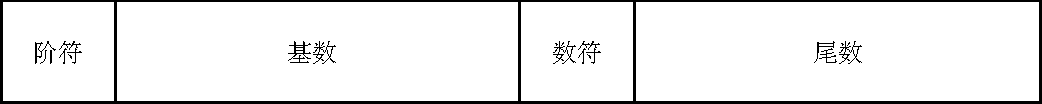
\includegraphics[scale=.7]{img/figure9.pdf}
\end{figure}
\subsection{浮点数的规格化}
规格化浮点数: 规定原码尾数的最高位一定要是个1$ \Leftrightarrow $ \texttt{|M|}属于\verb|[0.5,1]|, 所以衍生出以下两种规范化的方法:
\begin{itemize}
\item 左规: 说明\texttt{M<1/2}, 太小, 需要扩大, 左移\verb|1|位将尾数的数值位扩大到原来的\verb|2|倍, 同时阶码减\verb|1|
\item 右规: 说明\texttt{M>1}, 太大, 需要缩小, 右移\verb|1|位将尾数的数值位缩小到原来的\verb|1/2|倍, 同时阶码加\verb|1|
\end{itemize}\par
尾数可以用原码或者是补码表示, 所以上述左规和右规可以分别用于原码或者补码的规格化:
\begin{itemize}
\item 原码: 尾数最高位为\verb|1|
\begin{itemize}
\item 尾数为正数: 通过左规和右规得到的标准形式应该是\verb|0.1XXXXXXXX|
\item 尾数为负数: 通过左规和右规得到的标准形式应该是\verb|1.1XXXXXXXX|
\end{itemize}\par
注意, 上面尾数可以等于\verb|0.5|或者是\verb|-0.5|, 只要是\verb|0.1000000...|和\verb|1.1000000...|即可. 但是做不到等于\verb|1|或者\verb|-1|. 此外, 他们的数值位第一位都是\verb|1|, 所以在\hyperref[IEEE 754]{\texttt{IEEE 754}}中, 数值位的第一位可以默认省略.
\item 补码: 尾数最高位与符号位相反
\begin{itemize}
\item 尾数为正数: 通过左规和右规得到的标准形式应该是\verb|0.1XXXXXXXXX|
\item 尾数为负数: 通过左规和右规得到的标准形式应该是\verb|1.0XXXXXXXXX|
\end{itemize}
\end{itemize}
\subsection{\texttt{IEEE 754}标准}\label{IEEE 754} % TODO 阶码中的0和1有特殊用途, 以及IEEE表示范围
\begin{figure}[H]
\centering
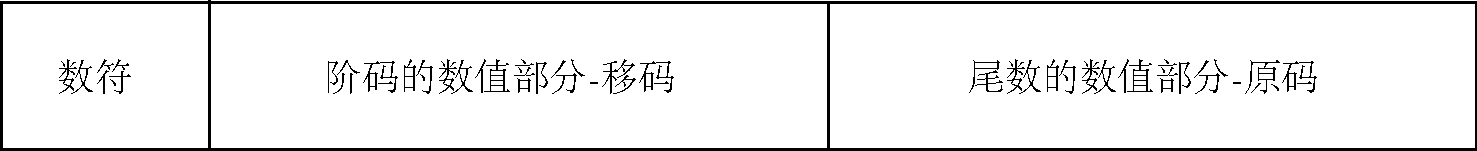
\includegraphics[scale=.5]{img/figure10.pdf}
\end{figure}
\subsubsection{阶码}
阶码用移码表示, 单精度浮点数下长度为\verb|8|位. \par
\hyperref[移码]{移码}是一种无符号数, 由于移码=真值+偏置值, 加完之后大于等于\verb|0|, 所以阶码没有符号位. 偏置值和数的类型有关, 单精度浮点数的偏置值为\verb|+127|, 双精度浮点数的偏置值为\verb|+1023|.
\subsubsection{尾数}
尾数用原码表示, 单精度浮点数下长度为\verb|23|位. \par
尾数是一种有符号数, 他的符号放在开头, 数值部分放在末尾. 通过规格化后, 数值部分默认隐藏首位\verb|1|, 所以单精度浮点数下实际能表示的数值位有\verb|24|位.
\subsubsection{举例}
以\verb|-1.75*2^(-3)|为例: \par
\begin{itemize}
\item 数符: 由于是负数, 所以是\verb|1|. \par
\item 尾数的数值部分: 十进制下是\verb|1.75>1|, 故需要右归, 尾数的数值部分右移\verb|1|位, 阶码需要加\verb|1|, 得到尾数的数值位为\verb|0.875|即\verb|1110000...(共24位)|, 阶码为\verb|-2|. 由于尾数的数值位的首位\verb|1|可以省略, 所以最终尾数的数值位为\verb|110000...(共23位)|. \par
\item 阶码: 经过上述规格化后, 阶码为\verb|-2|, 加上偏置值\verb|+127|, 得到移码十进制下为\verb|+125|, 转换为二进制为\verb|01111101|. \par
\end{itemize}
综上所述, 我们得到的\verb|IEEE 754|下的表示为: \verb|1,01111101,110000...(共23位)|.
\subsection{浮点数的加减运算}
我们通常在十进制下做浮点数的加减运算.
\subsubsection{步骤}
\begin{enumerate}
\item 对阶: 保持阶数一致, 小阶数向大阶数对齐
\item 尾数相加/减
\item 规格化, 保证尾数\verb|M|属于\verb|[0.5,1]|
\end{enumerate}
\subsubsection{举例}
实现\verb|0.75*2^4+1.5*2^3|:
\begin{enumerate}
\item 对阶: 小阶$ \rightarrow $大阶, \verb|1.5*2^3|$ \rightarrow $\verb|0.75*2^4|
\item 加减: \verb|0.75*2^4+0.75*2^4=1.5*2^4|
\item 规格化: \verb|1.5*2^4|$ \rightarrow $\verb|0.75*2^5|
\end{enumerate}
\chapter{存储器}
\section{存储器的层次}
\begin{figure}[H]
\centering
\begin{minipage}{.35\textwidth}
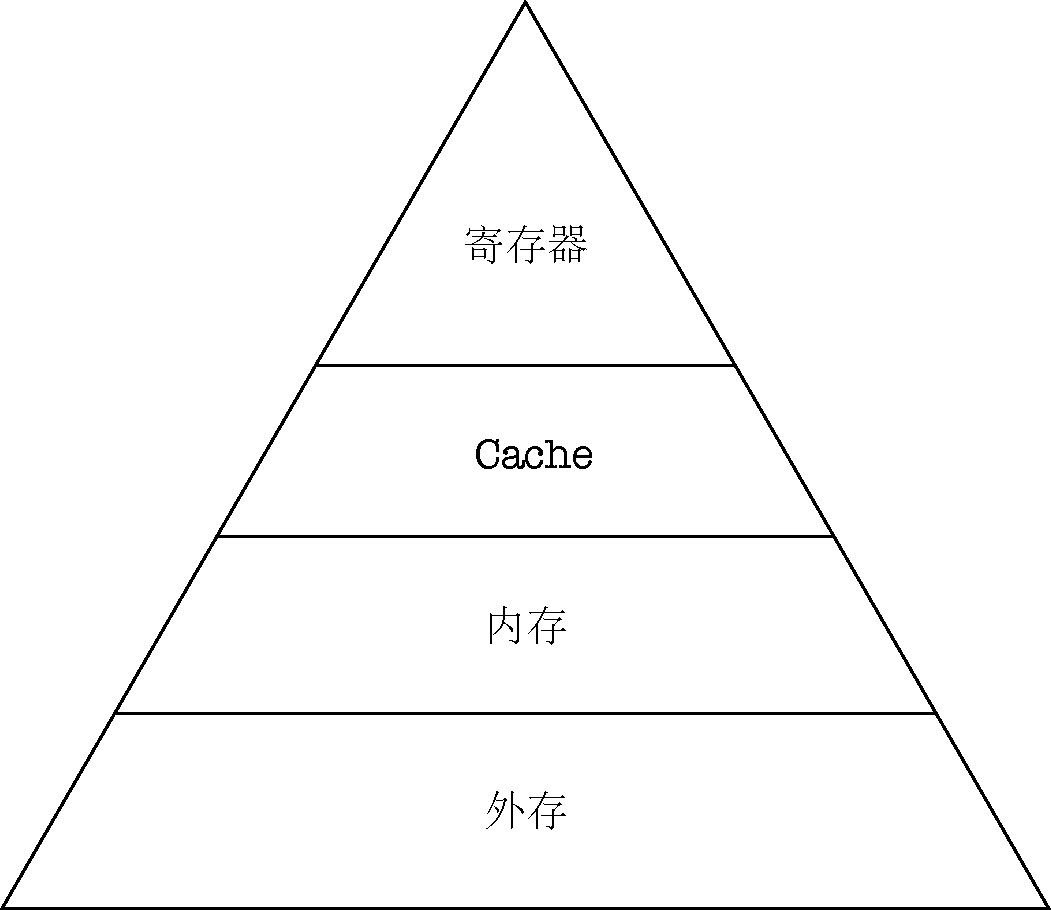
\includegraphics[scale=.3]{img/figure11.pdf}
\end{minipage}
\begin{minipage}{.48\textwidth}
\flushleft
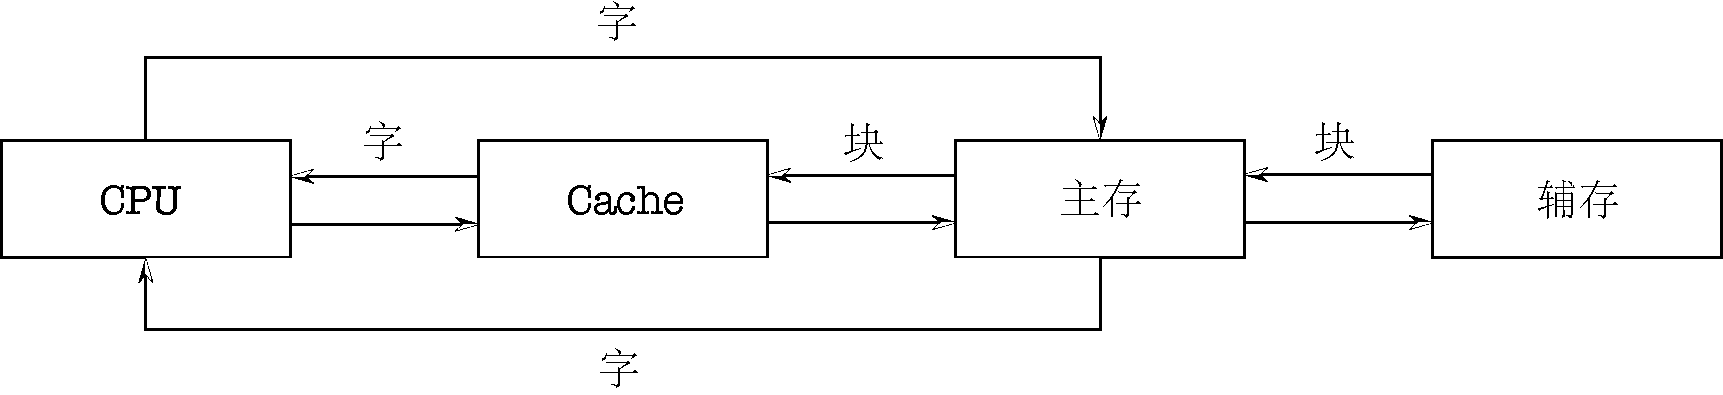
\includegraphics[scale=.3]{img/figure12.pdf}
\end{minipage}
\caption*{多级存储器结构}
\end{figure}
这就是存储器的层次结构. 在\verb|pyramid|的越上层, 价格越高, 速度越快, 容量越小. 要注意的是, \verb|Cache|和主存之间的数据交换是由硬件完成的, 对所有程序员透明. 主存和辅存之间的数据交换是由硬件和操作系统共同完成的. 对应用程序员透明.
\section{存储器的分类}
\begin{itemize}
\item 按层次分类
\begin{itemize}
\item 主存储器: 简称主存, 或者内存. 可以直接和\verb|Cache|交互
\item 辅助存储器: 简称辅存, 或者外存. 是主存的后援存储器
\item 高速缓冲存储器: 简称\verb|Cache|. 放在\verb|CPU|中
\end{itemize}
\item 按存取分类
\begin{itemize}
\item 随机存储器: \verb|RAM|, 可读可写, 存取时间和物理位置无关, 断电丢失数据
\begin{itemize}
\item 静态随机存储器: \verb|SRAM|, 双稳态触发器, 用于\verb|Cache|
\item 动态最急存储器: \verb|DRAM|, 栅极电容, 用于内存
\end{itemize}
\item 只读存储器: \verb|ROM|, 只读, 存取时间和物理位置无关, 断电不丢失数据
\item 串行访问存储器: 存储时间和物理位置有关, 如顺序存取存储器(磁带)与直接存取存储器(磁盘,光盘)
\end{itemize}
\item 按介质分类
分为: 磁表面存储器(磁盘,磁带), 磁芯存储器, 半导体存储器(MOS型存储器,双极型存储器)和光存储器(光盘)
\item 按可保存性分类
\begin{itemize}
\item 易失存储器: 断电后, 存储信息消失. 如: \verb|RAM|
\item 非易失存储器: 断电后, 存储信息依然保持, 如: \verb|ROM|
\item 破坏性读出: 某个存储单元被读出时, 原存储器信息被破坏
\item 非破坏性读出: 某个存储单元被读出时, 原存储器信息不会被破坏
\end{itemize}
\end{itemize}
\section{\texttt{Cache}}
\verb|Cache|是由\verb|SRAM|构成的, 在\verb|CPU|中的一种存储器.
\subsection{基本原理}
操作系统为了缓和\verb|CPU|和主存之间的速度矛盾, 将某些主存块放到了\verb|Cache|中, 而这个步骤是基于局部性原理:
\begin{itemize}
\item 时间局部性: 现在访问的地址, 不久之后也很可能再次被访问
\item 空间局部性: 现在访问的地址, 其附近的地址也很可能即将被访问
\end{itemize}
\subsection{性能分析}
\verb|CPU|访问数据有两种方式: 先访问\verb|Cache|, 若未命中再访问主存或者是同时访问\verb|Cache|和主存, 若命中\verb|Cache|则停止访问主存, 这就引出了\verb|Cache|的性能衡量标准:
\begin{itemize}
\item 命中率 \par 设\verb|Cache|的总命中次数为\verb|a|, 访问主存的次数为\verb|b|, 则命中率\verb|=a/(a+b)|
\item 缺失率 \par \verb|1-|命中率
\end{itemize}
\subsection{主存到\texttt{Cache}的映射}
\verb|Cache|被分成与主存的页框大小一致的\verb|Cache|块(或称Cache行), 两者之间以块为单位进行数据交换. 下面解释了内存中的块应该放在\verb|Cache|中的哪个位置:
\subsubsection{全相联映射}
主存的块可以装入\verb|Cache|的任何块, 没有公式. 相应的地址结构为:
\begin{figure}[H]
\centering
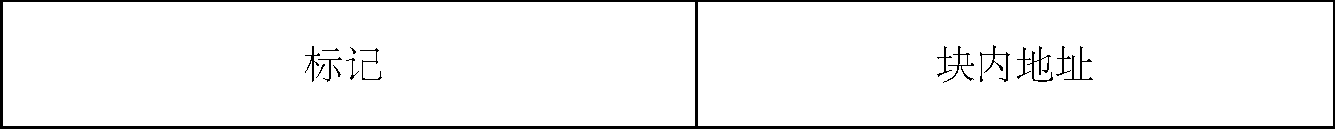
\includegraphics[scale=.5]{img/figure13.pdf}
\end{figure}
\subsubsection{直接映射}
主存中的块必须放入下面公式的指定\verb|Cache|块:
\begin{center}
\verb|j = i mod 2^c|, 其中\verb|j|为\verb|Cache|块号, \verb|i|为主存块号, \verb|2^c|为\verb|Cache|的总块数
\end{center} \par
\par 从上面的映射关系可以看出, 主存块号的低\verb|c|位正是它要装入的\verb|Cache|行号. 若主存中用\verb|m|位表示块号, 则标记(有效位+内存地址高位)共\verb|m-c|位, \verb|Cache|块号共\verb|c|位, 相应的地址结构为:
\begin{figure}[H]
\centering
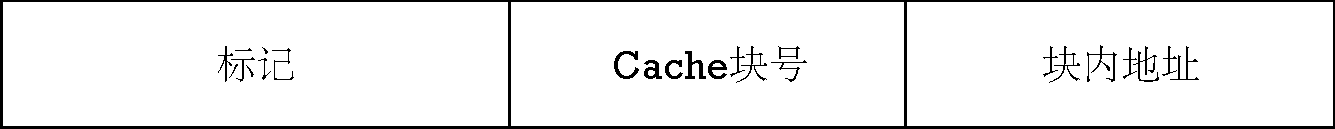
\includegraphics[scale=.5]{img/figure15.pdf}
\end{figure}\par
\subsubsection{组相联映射}
将\verb|Cache|分成大小相等的组, 主存的一个数据块可以装入一组内的任意位置, 即组间采取直接映射, 组内采取全相联映射, 内存块可以放在下面公式指定的\verb|Cache|\textbf{组}中:
\begin{center}
\verb|j = i mod Q|, 其中\verb|j|为\verb|Cache|块号, \verb|i|为主存块号, \verb|Q|为组数
\end{center}\par 
与直接映射相似, 主存块号的低位用来表示组号, 内存块号的高位和有效位用来表示标记, 相应的地址结构为:
\begin{figure}[H]
\centering
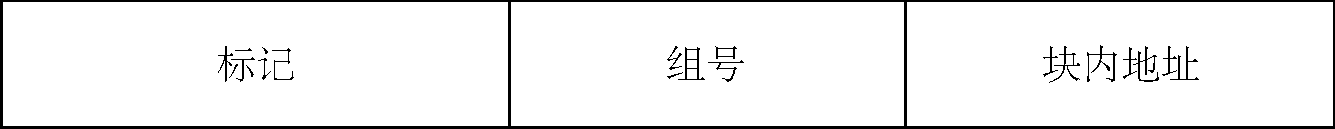
\includegraphics[scale=.5]{img/figure14.pdf}
\end{figure}
根据上述的地址结构, 我们应该可以推断出\verb|CPU|的访存过程:
\begin{figure}[H]
\centering
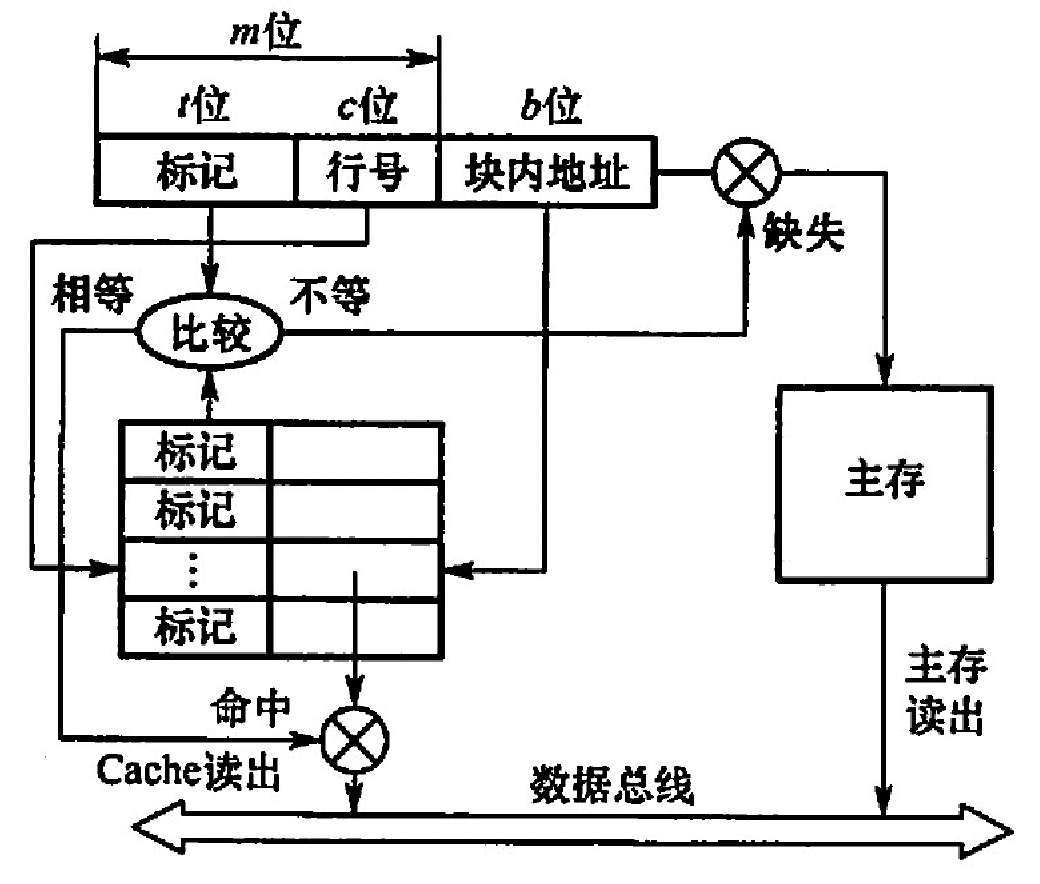
\includegraphics[scale=.45]{img/figure16.png}
\caption*{直接映射}
\end{figure}\par
上图为直接映射方式, 全相联映射中没有组,行号,内存地址高位低位的概念, 他的标记就是有效位+内存块号. 组相联映射是一种介于全相联映射和直接映射之间的一种映射.
\subsection{替换算法}
由于\verb|Cache|的空间通常很小, 所以用不到的\verb|Cache|块就要及时换出, 下面说明上述三种映射中替换算法要解决的问题:
\begin{itemize}
\item 全相联映射 \par \verb|Cache|满了才需要替换, 需要在全局选择替换哪一块
\item 直接映射 \par 如果对应位置非空, 则毫无选择地直接替换, 无需考虑替换算法
\item 组相联映射 \par 分组内满了才需要替换, 需要在分组内选择替换哪一块
\end{itemize}
\subsubsection{随机算法(\texttt{RAND})}
若\verb|Cache|已满, 则随机选择一块替换. \par
实现简单, 但是完全没有考虑局部性原理. 命中率低, 实际效果很不稳定.
\subsubsection{先进先出算法(\texttt{FIFO})}
若\verb|Cache|已满, 则替换最先被调入\verb|Cache|的块. \par
实现简单, 也是完全没有考虑局部性原理, 会出现抖动现象: 频繁的换入换出现象
\subsubsection{近期最少使用算法(\texttt{LRU})}
为每个\verb|Cache|设置一个``计数器'', 用于记录每个\verb|Cache|块已经多久没有被访问了, 当\verb|Cache|满后替换``计数器''最大的. \par
\begin{equation*}
y=|x|=
\scaleleftright[6pt]{\biggl\{}{
\begin{aligned}
& x,\ x\ge 0 \\
& -x,\ x<0
\end{aligned}
}{.}
\end{equation*}




